
\begin{tikzpicture}[-stealth,very thick,node distance = 4cm,auto]

	\node[state] (x) {$x$};
	\node[state] (y) [above right of=x] {$y$};
	\node[state] (z) [below right of=y] {$z$};
    
	\node[rectangle, minimum size=2em,draw] (a) [above left =of y] {$a$};
	\node[rectangle,minimum size=2em, draw] (b) [above = of y] {$b$};
	\node[rectangle, minimum size=2em,draw] (c) [above right =of y] {$c$};

	\draw[] (x) to node[above left] {$1$} (y);
	\draw[loop above] (y) to node {$0.5$} (y);
	\draw[bend left=20] (y) to node {$0.5$} (z);
	\draw[bend left=20] (z) to node[below left] {$0.7$} (y);
	\draw[] (z) to node {$0.3$} (x);
	
	\draw[dashed] (x) to node[left] {$0.9$} (a);
	\draw[dashed] (x) to node[left] {$0.1$} (b);
	\draw[bend right=30, dashed] (y) to node[right] {$0.6$} (b);
	\draw[dashed] (y) to node[below right] {$0.4$} (c);
	\draw[dashed] (z) to node[right] {$1$} (c);
	
	\node[rectangle, draw, scale=0.2, minimum size=20em,above = 2cm of a] (ga){\begin{tikzpicture}
			\begin{axis}[axis lines=none, ticks=none,xmax=3, xmin=-3,ymax=1.1]
				\addplot[ultra thick,black, no markers,samples=200] {exp(-x^2)};
			\end{axis}
		\end{tikzpicture}};
		
	\node[rectangle, draw, scale=0.2, minimum size=20em,above = 2cm of b] (gb){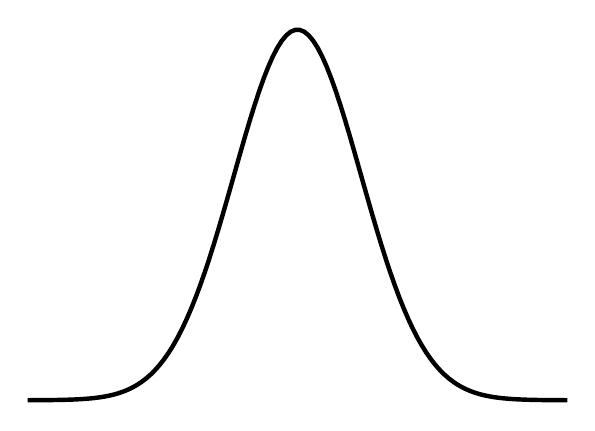
\begin{tikzpicture}
			\begin{axis}[axis lines=none, ticks=none,xmax=3, xmin=-3,ymax=1.1]
				\addplot[ultra thick,black, no markers,samples=200] {exp(-x^2)};
			\end{axis}
		\end{tikzpicture}};

	\node[rectangle, draw, scale=0.2, minimum size=20em,above = 2cm of c] (gc){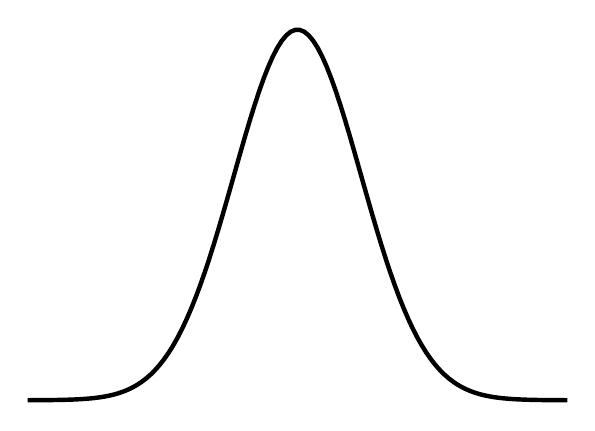
\begin{tikzpicture}
			\begin{axis}[axis lines=none, ticks=none,xmax=3, xmin=-3,ymax=1.1]
				\addplot[ultra thick,black, no markers,samples=200] {exp(-x^2)};
			\end{axis}
		\end{tikzpicture}};

	\draw[dotted, bend left] (a) to node[left] {$\mu_a$} (ga);
	\draw[dotted, bend right] (a) to node[right] {$\sigma_a$} (ga);
	\draw[dotted, bend left] (b) to node[left] {$\mu_b$} (gb);
	\draw[dotted, bend right] (b) to node[right] {$\sigma_b$} (gb);
	\draw[dotted, bend left] (c) to node[left] {$\mu_c$} (gc);
	\draw[dotted, bend right] (c) to node[right] {$\sigma_c$} (gc);

\end{tikzpicture}
